\chapter{Introduction}

\section{Overview}

PyLith is a multi-scale simulation software package for earthquake
physics. It is portable, scalable software for simulation of crustal
deformation across spatial scales ranging from meters to hundreds of
kilometers and temporal scales ranging from milliseconds to thousands
of years

\section{History}

This first version of PyLith is a direct descendant of Lithomop and
marks the first version that runs in parallel. Lithomop was the
product of major reengineering of Tecton, a finite-element code for
simulating static and quasi-static crustal deformation. The major new
features present in Lithomop included dynamic memory allocation and
the use of the Pyre simulation framework and PETSc solvers. </para>
<para> PyLith is currently being rewritten from scratch to create a
much more modular, powerful simulation package. This new code will
include earthquake dynamics (both rupture propagation and seismic wave
propagation). A beta release is expected in late 2006.

\section{Governing Equations}

Both LithoMop3d and PyLith-0.8 are quasi-static codes, meaning that
time-dependence only enters through the constitutive relationships and
the loading conditions. The description here is for the small-strain
formulation, which is the only formulation available at present. If a
large deformation solution is desired, interested users may contact
Charles Williams (willic3@rpi.edu) about a version of the finite
element code TECTON.

The problem is formulated in terms of the stresses ($\sigma_{ij}$),
displacements ($u_i$), and body forces per unit volume
(figs/g-inlineeq1.eps). We use standard index notation for all
equations here, such that repeated indices imply summation and a comma
denotes differentiation. For a general three-dimensional body, the
problem must satisfy the equilibrium conditions
\begin{equation}
  \text{figs/g-eq1.eps}
\end{equation}
subject to the natural boundary conditions
\begin{equation}
  \text{figs/g-eq2.eps}
\end{equation}
and the essential boundary conditions
\begin{equation}
  \text{figs/g-eq3.eps}
\end{equation}
The surface of the body is $S$, given by
\begin{equation}
  \text{figs/g-eq4.eps}
\end{equation}
The $n_j$ are the components of the unit normal vector to $S$, the
\begin{equation}
  \text{figs/g-inlineeq2.eps}
\end{equation}
are the components of the surface tractions, and the 
\begin{equation}
  \text{figs/g-inlineeq3.eps}
\end{equation}
are the components of the applied displacements. The stresses are
computed from the strains and any existing initial stresses using a
given constitutive relationship. The strains are given by
\begin{equation}
\text{figs/g-eq5.eps}  
\end{equation}
For a linear elastic material, the constitutive relationship between
stress and strain is
\begin{equation}
  \text{figs/g-eq6.eps}
\end{equation}
where
\begin{equation}
  \text{figs/g-inlineeq4.eps}
\end{equation}
are the initial stresses, and $C$
\begin{equation}
  \text{g-inlineeq5.eps}
\end{equation}
is the elastic constitutive relation.

For inelastic behavior (viscous, plastic, etc.), we assume an additive
decomposition of the strain tensor into elastic and inelastic parts,
and use an integrated form of the classical incremental theory of
plasticity. At time $t+\Delta t$, he stresses are therefore computed
from the total elastic strain:
\begin{equation}
  \text{figs/g-eq7.eps}
\end{equation}
where
\begin{equation}
  \text{figs/g-inlineeq6.eps}
\end{equation}
are the total strains and
\begin{equation}
  \text{figs/g-inlineeq7.eps}
\end{equation}
are the inelastic strains, with the difference being the elastic
strains. In our actual computations, we use a formulation that
decomposes the stresses into the deviatoric and volumetric parts,
using ideas based on the "effective stress function"
\cite{Kojic:Bathe:1987}. This allows the time integration of stresses
to be performed in terms of a single parameter related to the second
deviatoric stress invariant.

\section{Software Components}

PyLith is separated into modules to encapsulate behavior and
facilitate use across multiple applications. That way expert users can
replace functionality of a wide variety of components without
recompiling or polluting the main code. External packages reduce
development time and enhance computational efficiency, for example,
PyLith runs 2x faster by using the PETSc linear solver.

PyLith is based on several programming languages. High-level code is
written in Python; this rich, expressive interpreted language with
dynamic typing reduces development time. Low-level code is written in
Fortran 77 for fast execution. Bindings, written in C/C++, are used to
allow the low-level code (Fortran 77) to be called from high-level
code (Python).

PyLith makes extensive use of external software. Pyre is a science
neutral simulation framework being developed at Caltech. PETSc is used
to perform operations on matrices and vectors in parallel.

\subsection{PETSc}

\href{http://www-unix.mcs.anl.gov/petsc/petsc-as/}{PETSc}, the
Portable, Extensible Toolkit for Scientific computation, provides a
suite of routines for parallel, numerical solution of partial
differential equations for linear and nonlinear systems with large,
sparse systems of equations. PETSc includes solvers that implement a
variety of Newton and Krylov subspace methods. It can also interface
with many external packages, including BlockSolve95, ESSL, Matlab,
ParMeTis, PVODE, and SPAI, thereby providing additional solvers and
interaction with other software packages.

PETSc includes interfaces for Fortran, C, and C++ for nearly all of
the routines and PETSc can be installed on most Unix systems. PETSc
can be built with user supplied highly optimized linear algebra
routines (e.g., ATLAS and commercial versions of BLAS/LAPACK), thereby
improving application performance. Users can use PETSc parallel
matrices, vectors, and other data structures for most parallel
operations, eliminating the need for explicit calls to Message Passing
Interface (MPI) routines. Many settings and options can be controlled
with PETSc specific command-line arguments, including selection of
preconditions, solvers, and generation of performance logs.

\subsection{Pyre}

Pyre is an object-oriented environment capable of specifying and
launching numerical simulations on multiple platforms, including
Beowulf class parallel computers and grid computing systems. Pyre
allows the binding of multiple components such as solid and fluid
models used in Earth science simulations, and different meshers. The
Pyre framework enables the elegant setup, modification and launching
of massively parallel three-dimensional solver applications.

Pyre is a framework, a combination of software and design philosophy
that promotes the reuse of code. In their canonical software design
book, {\em Design Patterns}, Erich Gamma {\it et al}.  condense the
concept of a framework concept down to, "When you use a framework, you
reuse the main body and write the code it calls." In the context of
frameworks and object-oriented programming, Pyre can be thought of as
a collection of classes and the way their instances interact.
Programming applications based on Pyre will look similar to those
written in any other object-oriented language. The Pyre framework
contains a subset of parts that make up the overall framework. Each of
those parts is designed to solve a specific problem.

The framework approach to computation offers many advantages. It
permits the exchange of codes and promotes the reuse of standardized
software while preserving efficiency. Frameworks are also an efficient
way to handle changes in computer architecture. They present
programmers and scientists with a unified and well-defined task and
allow for shared costs of the housekeeping aspects of software
development. They provide greater institutional continuity to model
development than piecemeal approaches.


The Pyre framework incorporates features aimed at enabling the
scientific non-expert to perform tasks easily without hindering the
expert. Target features for end users allow complete and intuitive
simulation specification, reasonable defaults, consistency checks of
input, good diagnostics, easy access to remote facilities, and status
monitoring. Target features for developers include easy access to user
input, a shorter development cycle, and good debugging support.

\begin{figure}[htbp]
  \begin{center}
    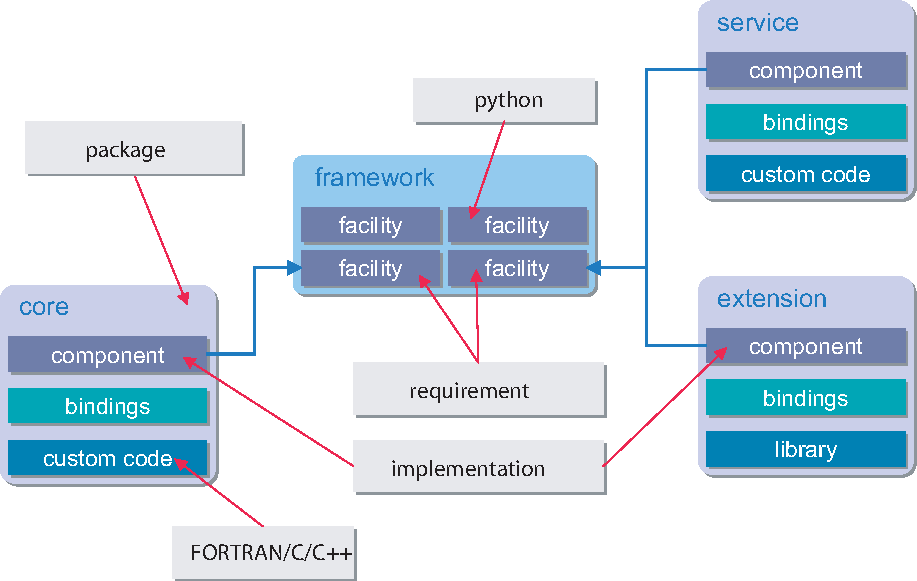
\includegraphics[scale=0.75]{figs/pyre_overview}
    \caption{Pyre Architecture. The integration framework is a set of
      cooperating abstract services.}
  \end{center}
\end{figure}

\section{PyLith Design}

In transforming Lithomop, a serial code, into PyLith, a parallel code,
a principal concern was to preserve the existing structure of the
serial Fortran code. Active development of purely analytic features in
PyLith, such as new material models or discretization schemes, depends
on the familiarity of application scientists with the traditional
Fortran programming paradigm. Global, topological operation should be
strictly segregated from the existing code. In fact, with the
exception of integrating PETSc for serial linear algebra and solver
operations, PyLith can be run purely in serial without activating any
of the parallel capabilities.

In order to accomplish this separation, we use the PETSc
\classname{Sieve} structure to create a model of the serial
PyLith mesh. This model is then partitioned and distributed to a set
of processes. Each process receives a self-consistent mesh, meaning
the pieces are overlapping. Each process then executes a serial PyLith
step on that particular mesh piece. The PETSc linear algebra
operations are overloaded, using the \classname{Sieve}
information, to produce a globally consistent field.

